\chapter{Supplementary Figures and Tables}

This section contains all the supplemental figures and tables for Chapters~\ref{chapter:deprescribing}, \ref{chapter:race-bayes}, and \ref{chapter:bn-reasoning}. 

\section{Aim 1: Supplementary Figures}

\begin{figure}[ht!]
	\centering
	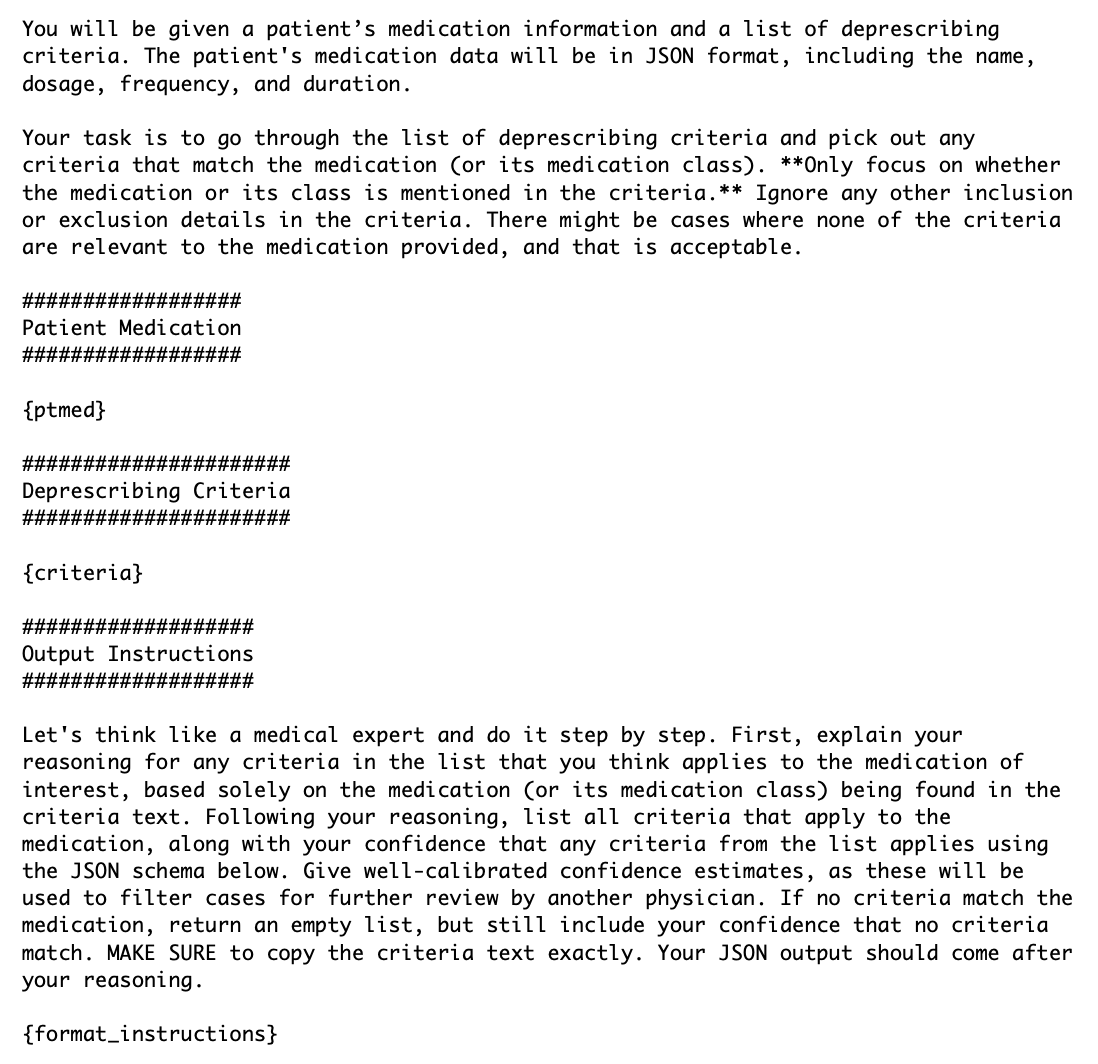
\includegraphics[width=\textwidth] {figures/aim1/step1_prompt.png}
	\caption{Prompt for Step 1 (Eligibility Filtering). \texttt{ptmed} is a single med from a patient’s outpatient medication list, \texttt{criteria} is the full list of high-yield criteria to be filtered, and \texttt{format\_instructions} are the instructions to output the relevant, filtered criteria and confidence in a structured JSON format.} \label{fig:aim1-step1-prompt}
\end{figure}

\begin{figure}[ht!]
	\centering
	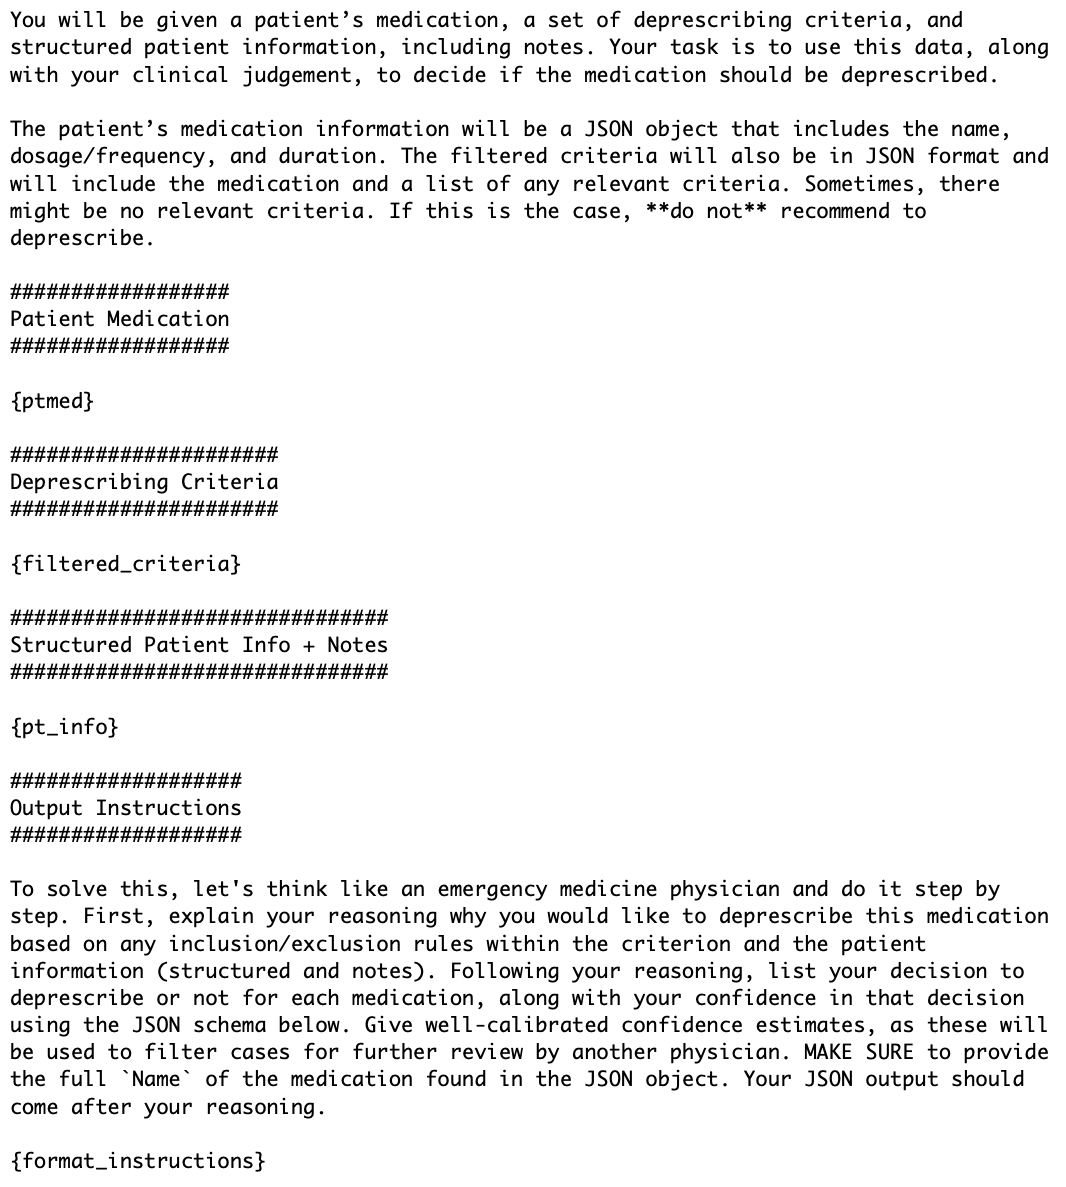
\includegraphics[width=\textwidth] {figures/aim1/step2_prompt.png}
	\caption{Prompt for Step 2 (Deprescribing Recommendations). \texttt{ptmed} is a single med from a patient’s outpatient medication list, \texttt{filtered\_criteria} is the list of filtered high-yield criteria from Step 1, \texttt{pt\_info} is the formatted text of the structured patient information and most recent progress note and discharge summary with delimiters, and \texttt{format\_instructions} are the instructions to output the deprescribing recommendation and confidence in a structured JSON format.} \label{fig:aim1-step2-prompt}
\end{figure}


\begin{figure}[ht!]
	\centering
	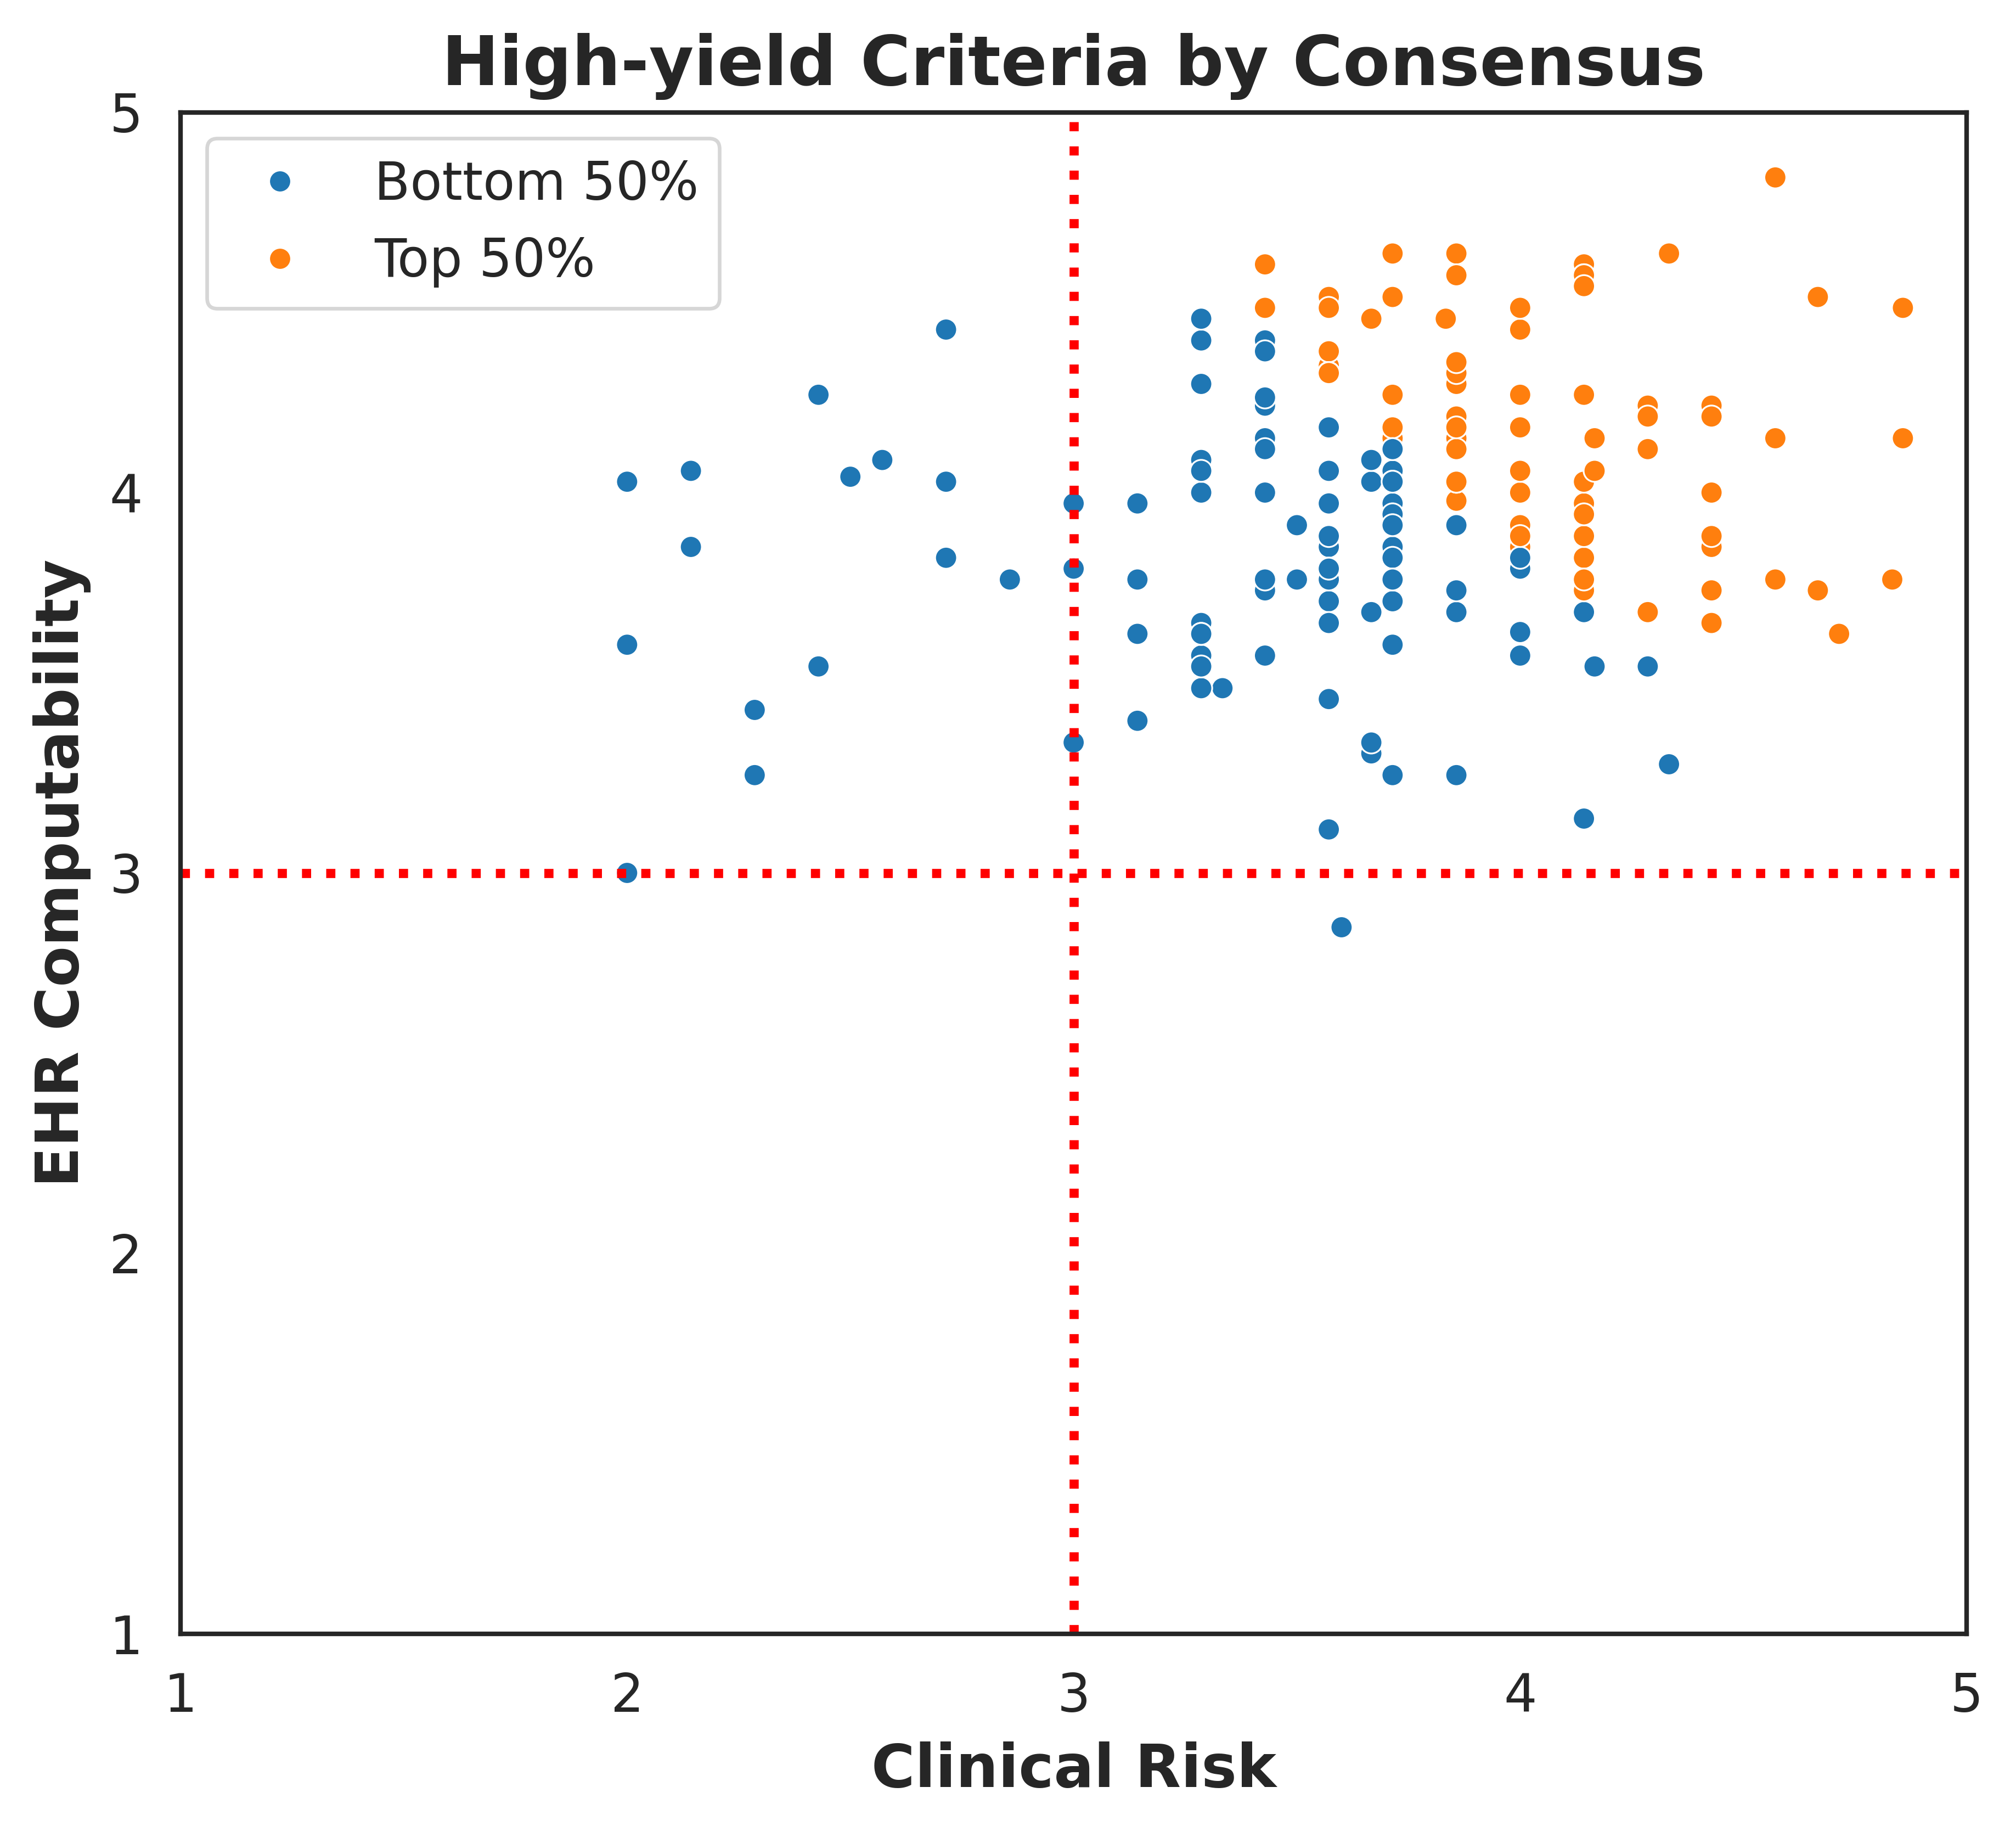
\includegraphics[width=\textwidth] {figures/aim1/consensus_study_avg_ratings.png}
	\caption{Selected deprescribing criteria as a function of patient risk and Electronic Health Record (EHR) computability from the consensus-based evaluation of Screening Tool of Older People’s Prescriptions (STOPP), Beers, and GEMS-Rx. Red dotted lines indicate cutoffs at clinical risk >3 and EHR computability >3. Given the large number of criteria still within the upper right quadrant (potentially high yield), the top 50\% of the quadrant was selected (orange) as the final list.} \label{fig:aim1-consensus-avg-ratings}
\end{figure}


\begin{figure}[ht!]
	\centering
	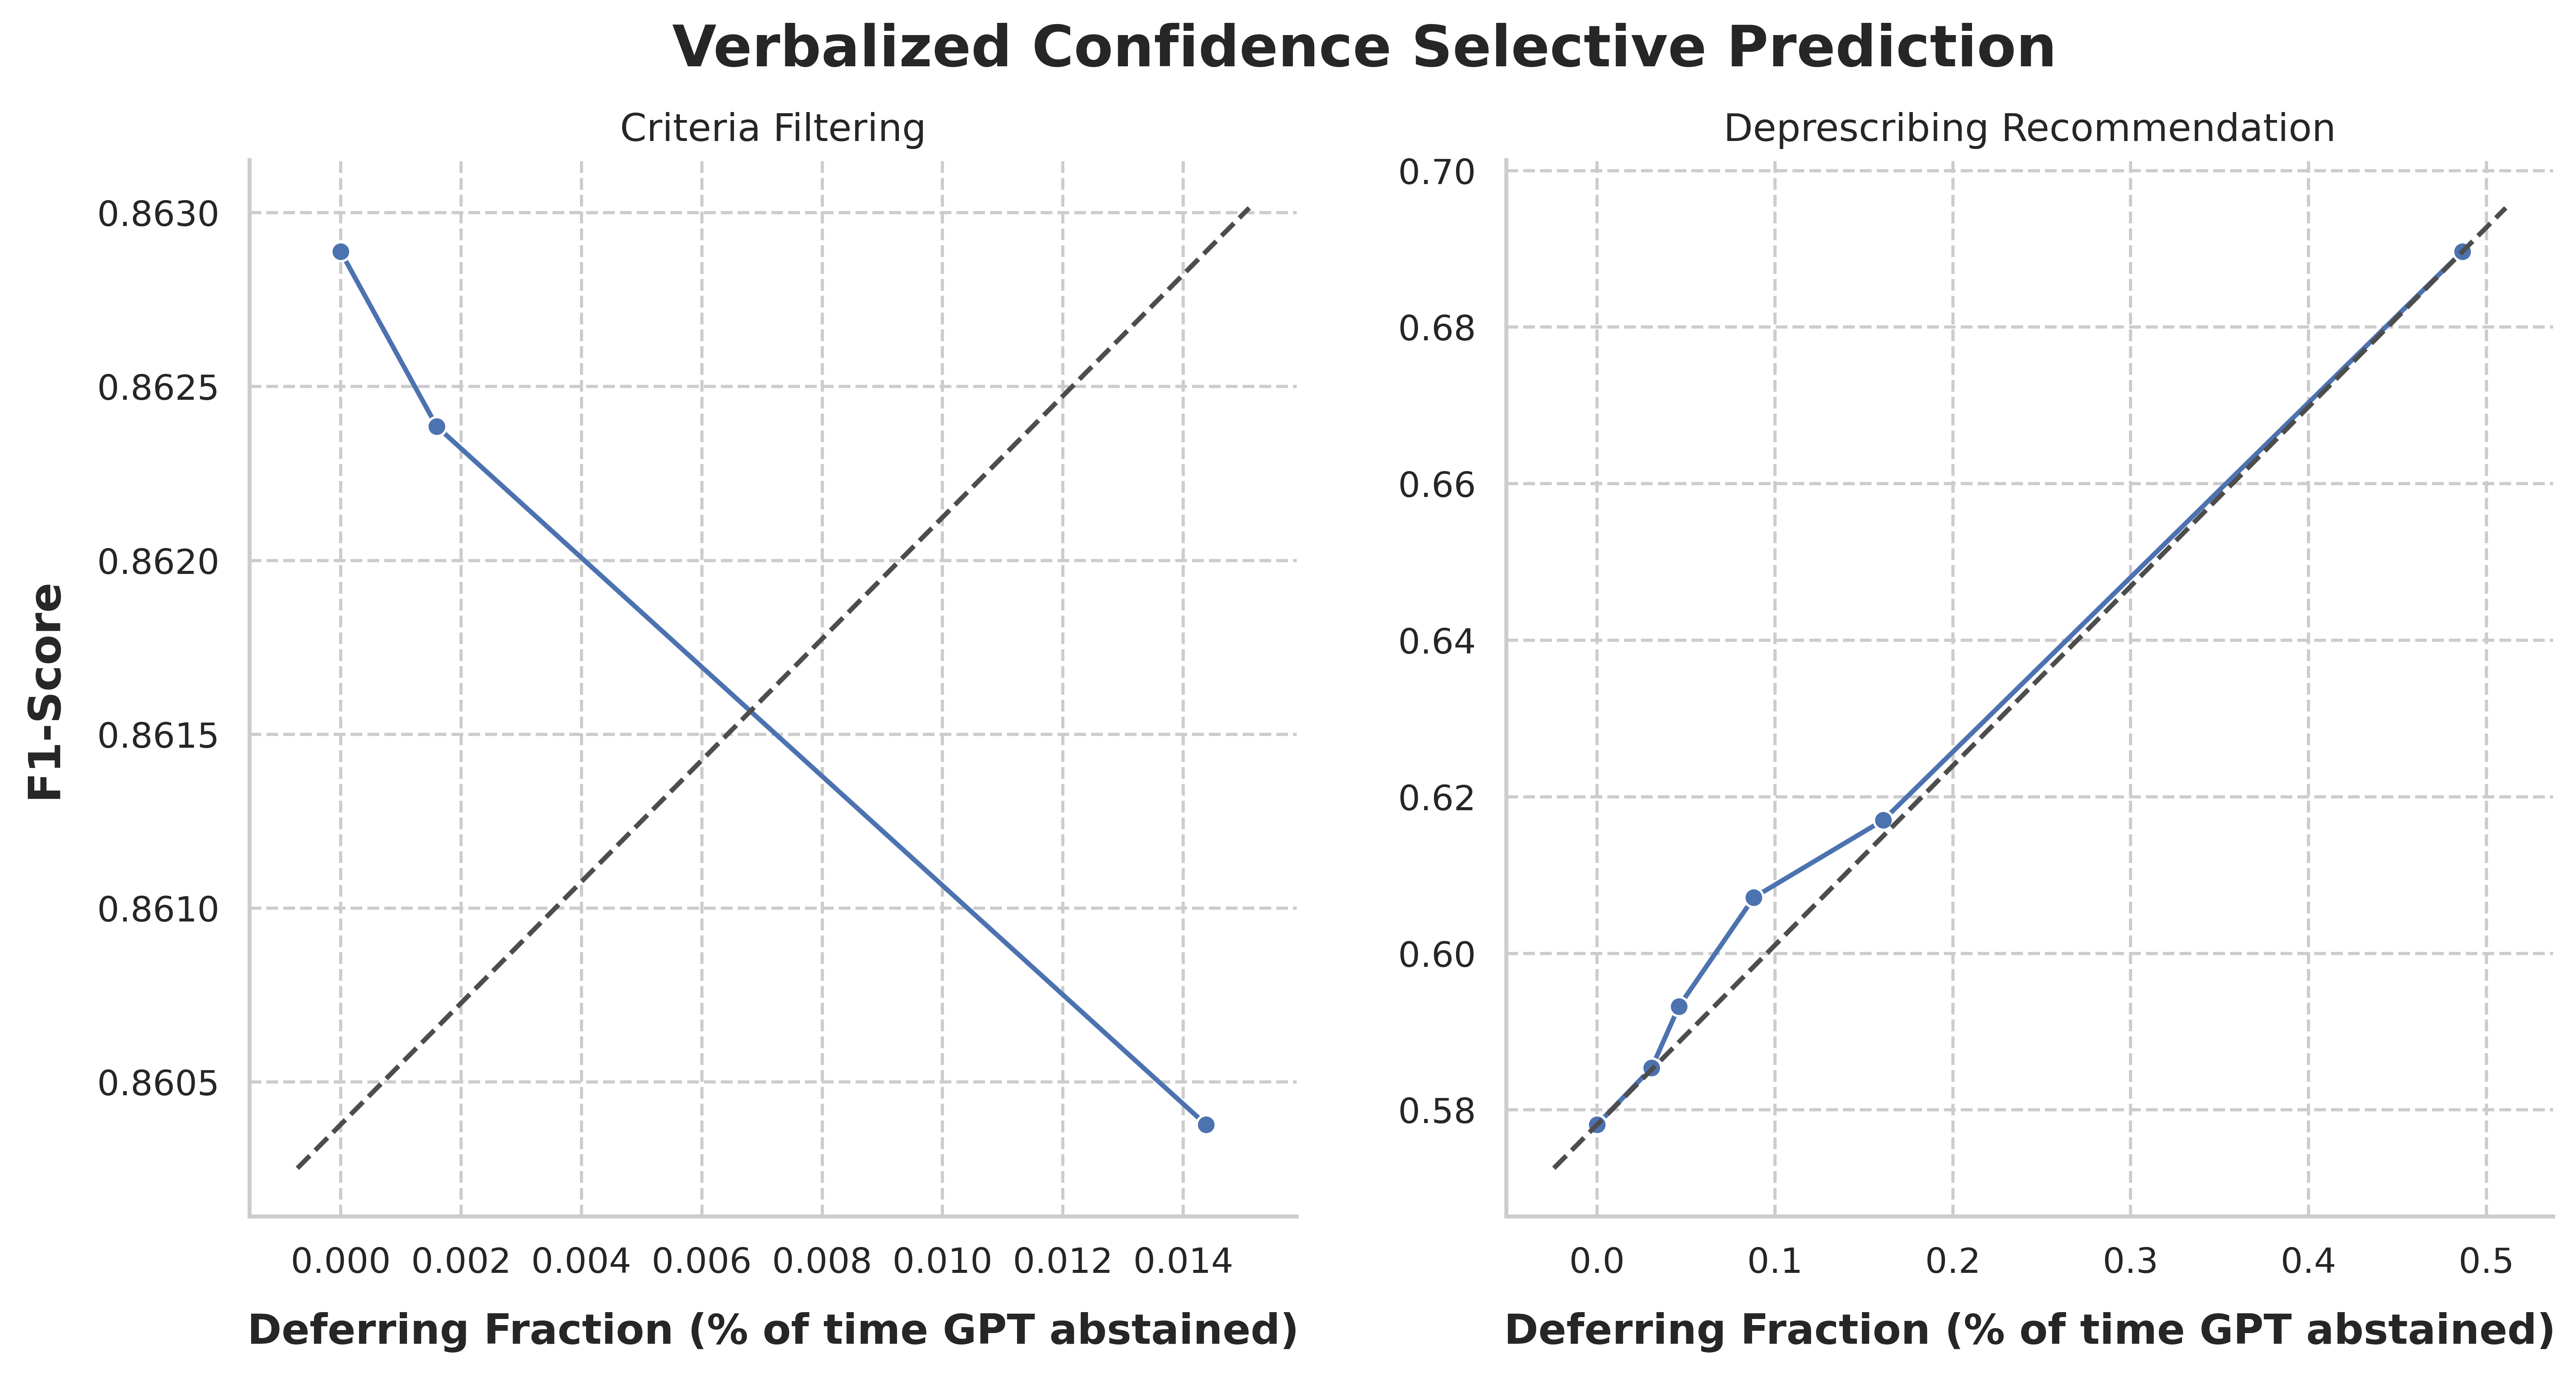
\includegraphics[width=\textwidth] {figures/aim1/selective_pred_verbconf.png}
	\caption{Range of F1-scores resulting from the application of verbalized confidence-based selective prediction for both steps of the deprescribing pipeline. The dotted line shows ideal performance as a function of deferring fraction.} \label{fig:aim1-verbconf}
\end{figure}

\section{Aim 3: Supplementary Figures}

\begin{figure}[ht!]
	\centering
	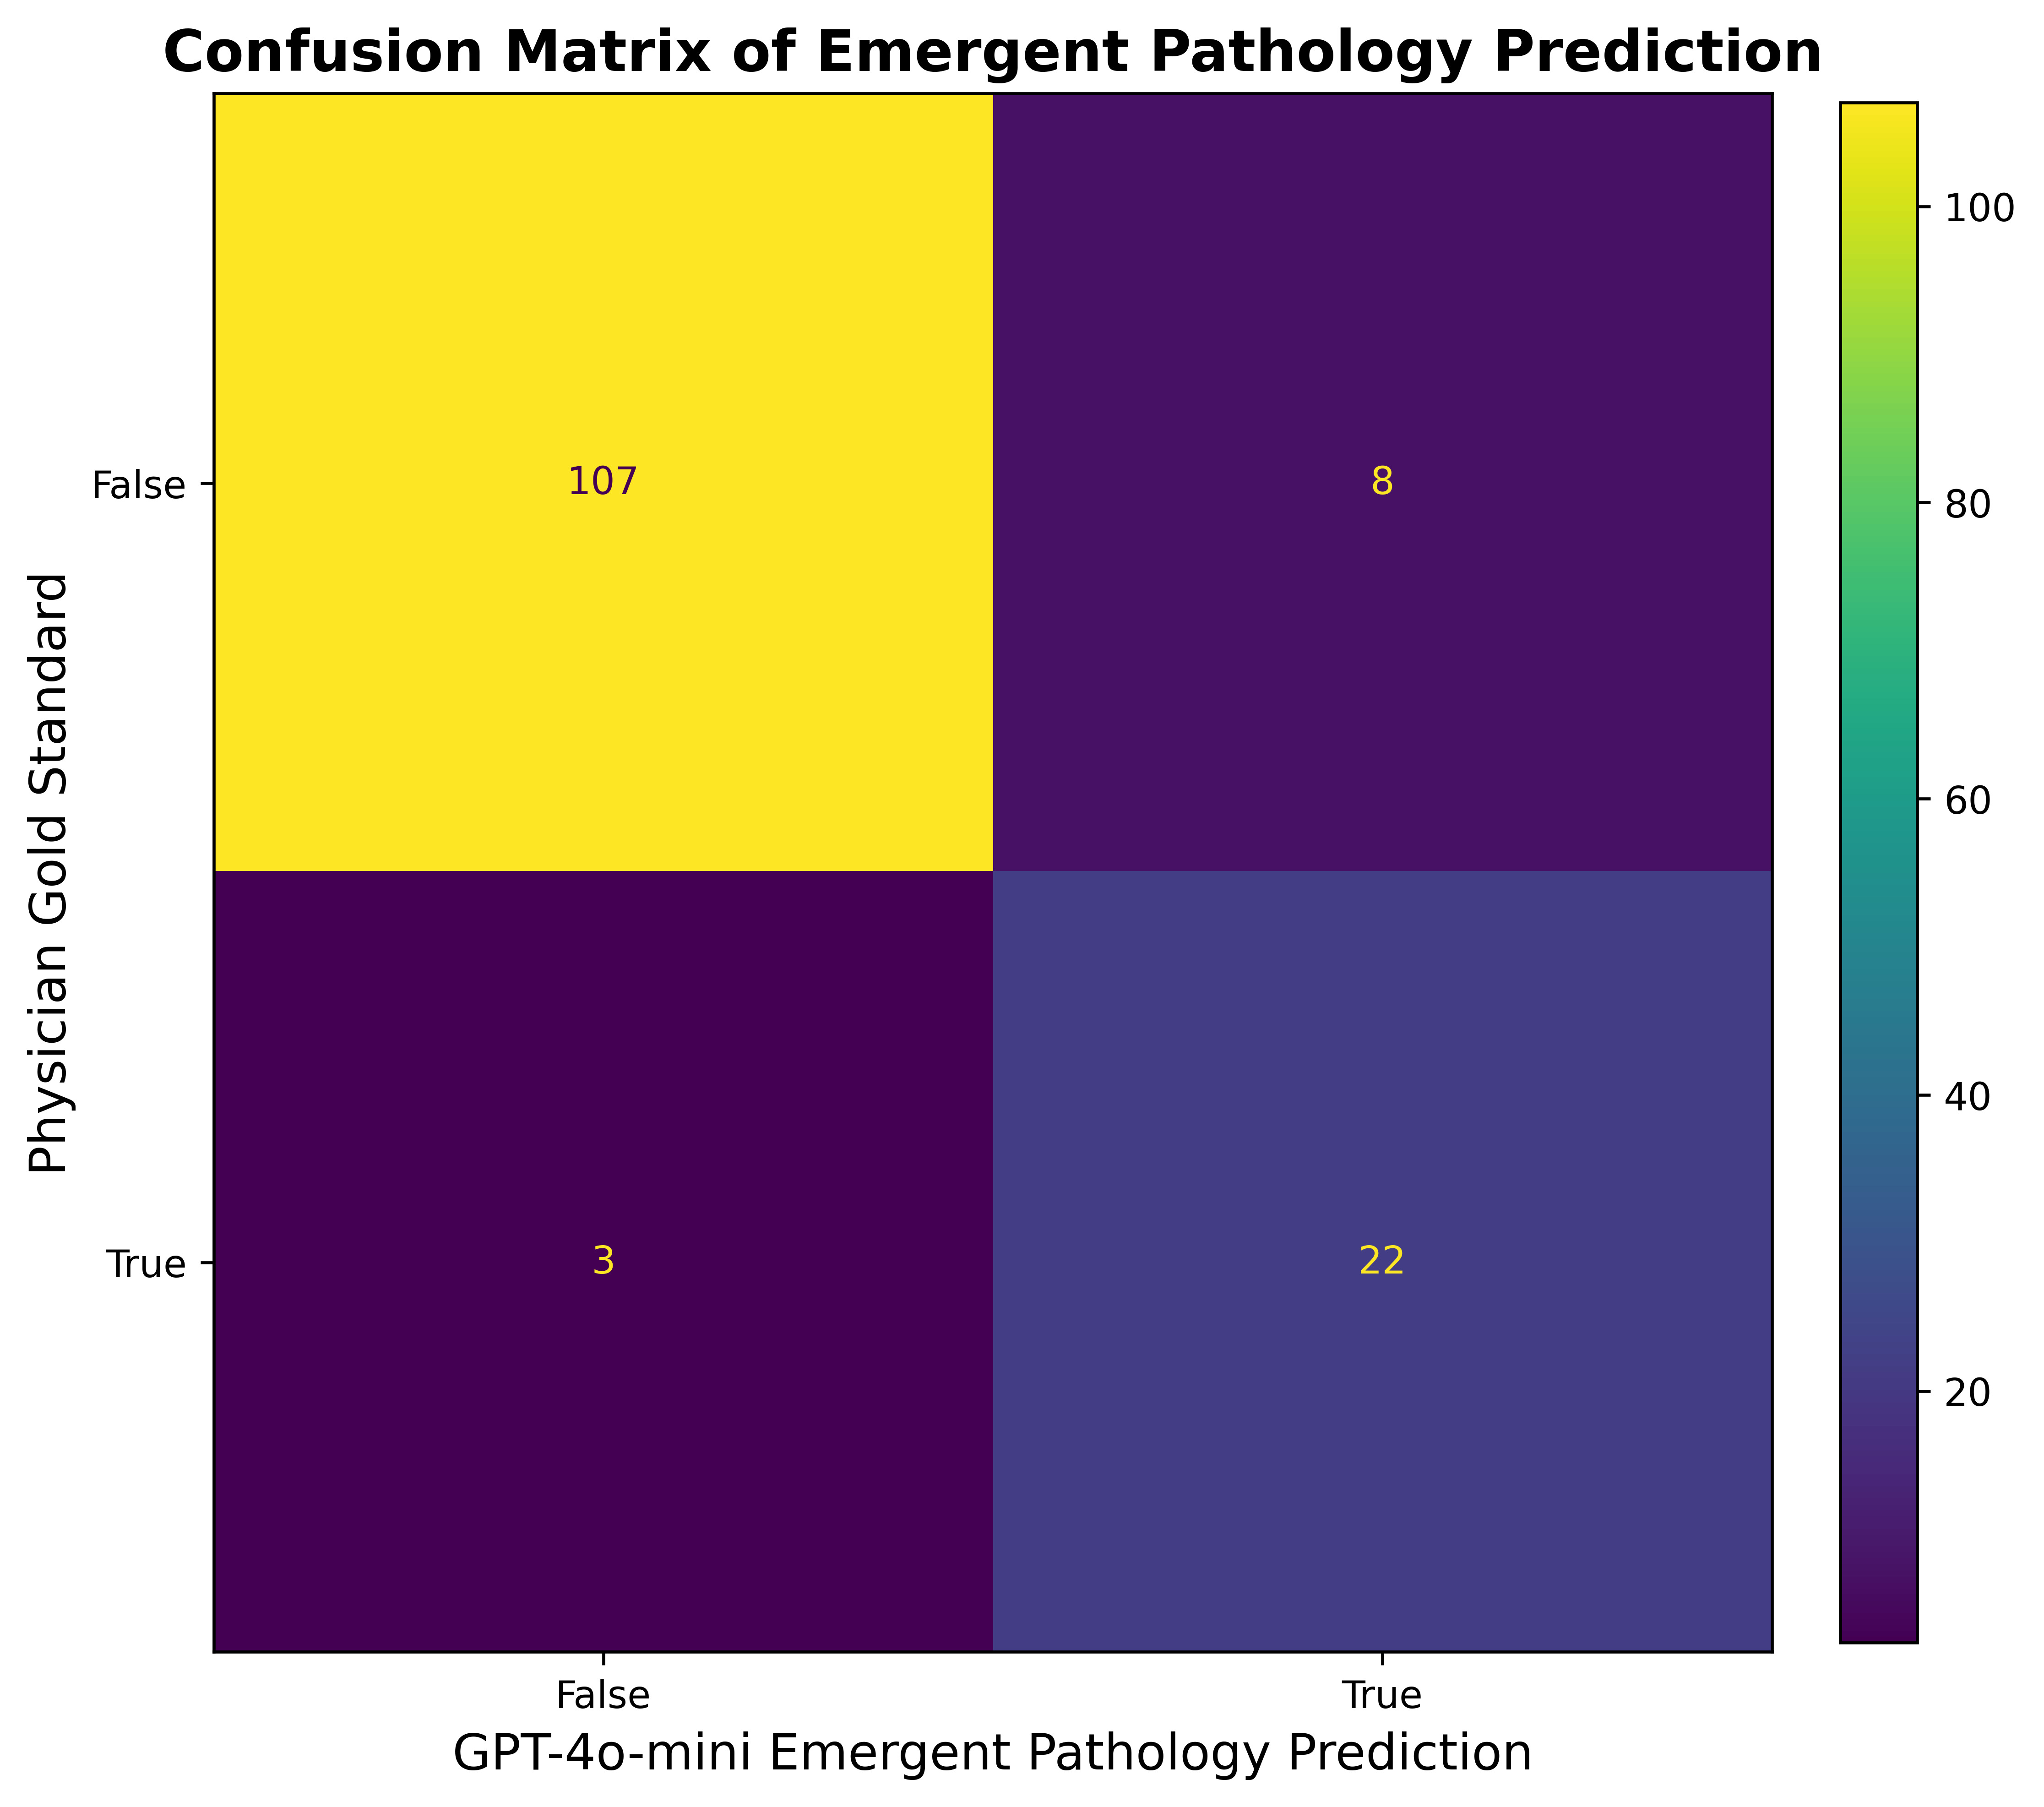
\includegraphics[width=0.85\textwidth] {figures/aim3/imaging_emergent_path_confmat.png}
	\caption{Confusion matrix comparing GPT-4o-mini's prediction of emergent pathology findings in radiology consults, compared with gold-standard physician annotations.} \label{fig:aim3-imaging-path-confmat}
\end{figure}


\begin{figure}[ht!]
	\centering
	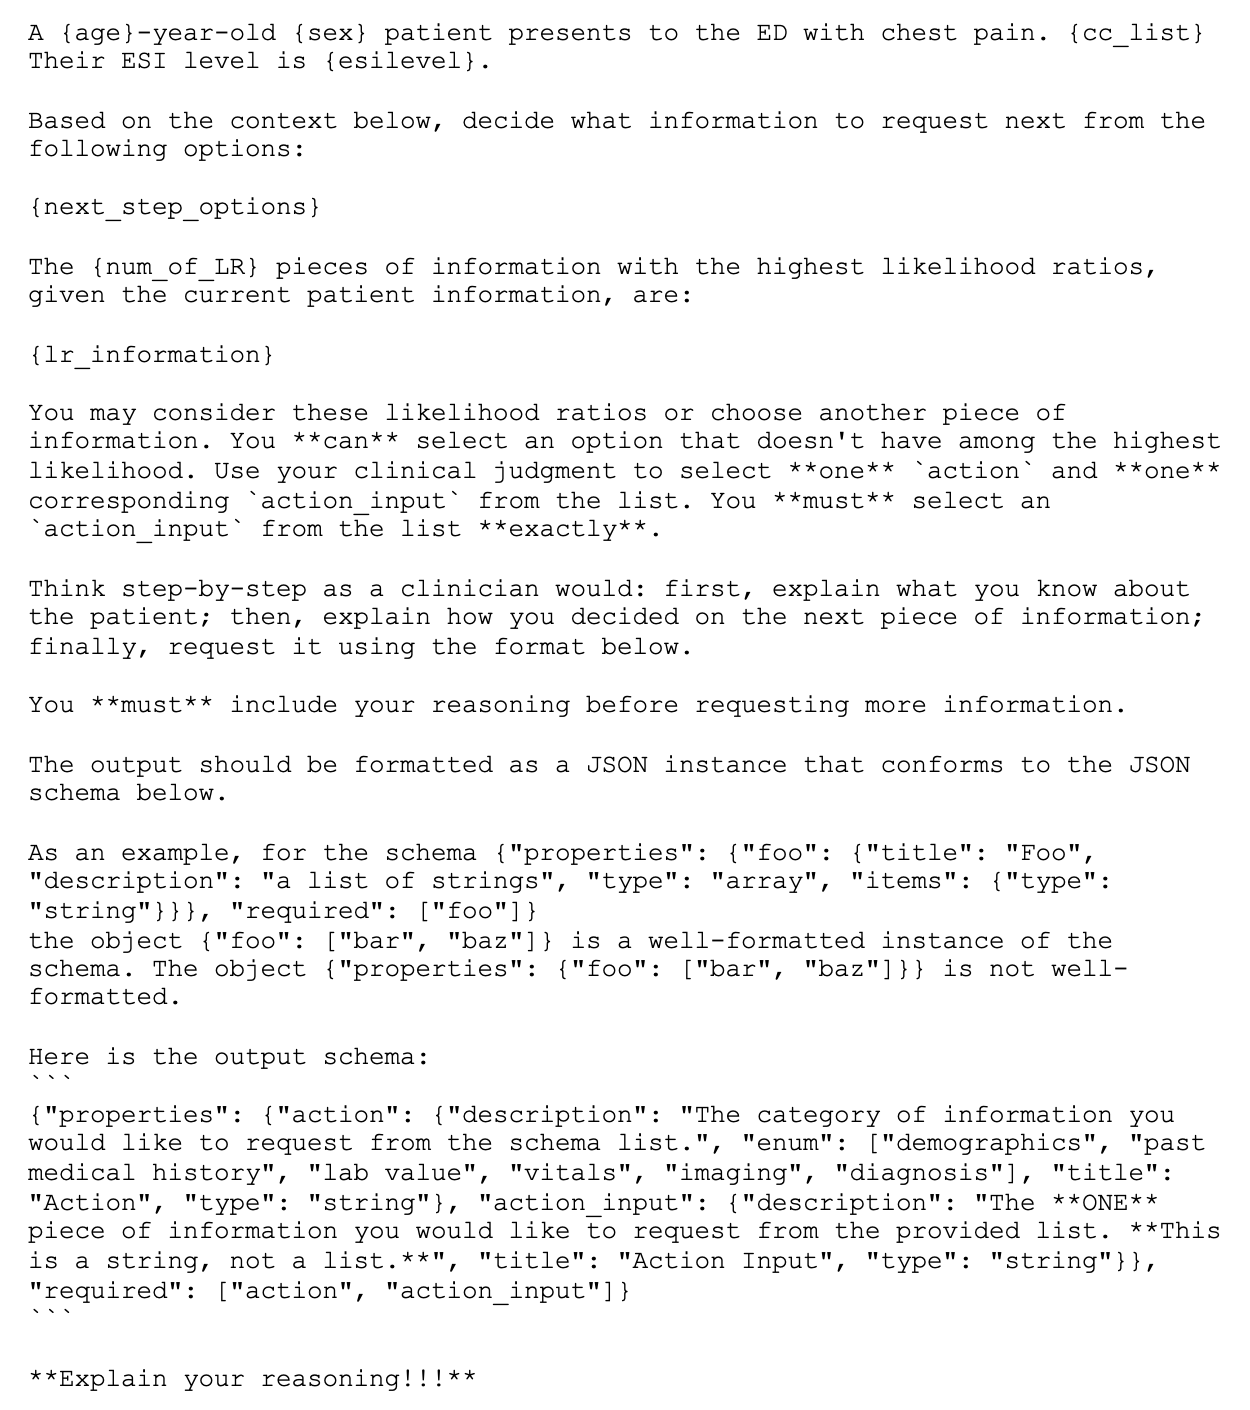
\includegraphics[width=0.85\textwidth] {figures/aim3/intro_prompt.png}
	\caption{Diagnostic conversation prompt providing triage information, available data elements to request, and formatting instructions to request an \texttt{action} and \texttt{action\_input}.} \label{fig:aim3-prompt}
\end{figure}

\setlength\LTleft{0pt}
\setlength\LTright{0pt}
\begin{longtable}{@{\extracolsep{\fill}}lll}
\caption{All data columns used in training the Bayesian network and available to the LLM for diagnostic conversations.}\label{tab:aim3-data-columns1}\\

\hline
Column \# & Data Column & Description \\
\hline
\endhead

\hline
\endfoot
0 & PAT\_ENC\_CSN\_ID & CSN \\
1 & Acute\_Coronary\_Syndrome & Acute Coronary Syndrome \\
2 & Pulmonary\_Embolism & Pulmonary Embolism \\
3 & Aortic\_Dissection & Aortic Dissection \\
4 & Pneumonia & Pneumonia \\
5 & Esophageal\_Rupture & Esophageal Rupture \\
6 & Pneumothorax & Pneumothorax \\
7 & Pericarditis & Pericarditis \\
8 & ESI & ESI \\
9 & Age & age \\
10 & Sex & sex \\
11 & Race & race \\
12 & Ethnicity & ethnicity \\
13 & Smoking\_Status & smoking status \\
14 & CC\_abdominal\_pain & chief complaint of abdominal pain \\
15 & CC\_alcohol\_intoxication & chief complaint of  alcohol intoxification \\
16 & CC\_back\_pain & chief complaint of back pain \\
17 & CC\_chest\_pain & chief complaint of chest pain \\
18 & CC\_cough & chief complaint of cough \\
19 & CC\_diarrhea & chief complaint of diarrhea \\
20 & CC\_dizziness & chief complaint of dizziness \\
21 & CC\_emesis & chief complaint of emesis \\
22 & CC\_fall & chief complaint of fall \\
23 & CC\_fever & chief complaint of fever \\
24 & CC\_headache & chief complaint of headache \\
25 & CC\_leg\_pain & chief complaint of leg pain \\
26 & CC\_motor\_vehicle\_crash & chief complaint of motor vehicle crash \\
27 & CC\_nausea & chief complaint of nausea \\
28 & CC\_rash & chief complaint of rash \\
29 & CC\_shortness\_of\_breath & chief complaint of shortness of breath \\
30 & CC\_sore\_throat & chief complaint of sore throat \\
31 & CC\_suicidal & chief complaint of suicidal thoughts \\
32 & CC\_weakness & chief complaint of weakness \\
33 & Hx\_abdominal\_pain & history of abdominal pain \\
34 & Hx\_allergy & history of allergy \\
35 & Hx\_anemia & history of anemia \\
36 & Hx\_anxiety\_dx & history of anxiety disorders \\
37 & Hx\_asthma & history of asthma \\
38 & Hx\_back\_problem & history of back problems \\
39 & Hx\_breast\_dx & history of breast disorders \\
40 & Hx\_chest\_pain & history of nonspecific chest pain \\
41 & Hx\_COPD & history of COPD \\
42 & Hx\_atherosclerosis\_other\_heart\_dx & history of Coronary atherosclerosis and/or other heart disease \\
43 & Hx\_DM & history of Diabetes mellitus without complication \\
44 & Hx\_dizziness & history of conditions associated with dizziness or vertigo \\
45 & Hx\_dysrhythmia & history of cardiac dysrhythmias \\
46 & Hx\_fall & history of falls \\
47 & Hx\_esophgeal\_dx & history of esophageal disorders \\
48 & Hx\_fatigue & history of malaise and fatigue \\
49 & Hx\_fluid\_electrolyte\_dx & history of fluid and electrolyte disorders \\
50 & Hx\_headache\_migraines & history of headaches and/or migraines \\
51 & Hx\_HTN & history of essential hypertension \\
52 & Hx\_lipid\_metabolism\_dx & history of hyperlipidemia \\
53 & Hx\_immunizations\_infec\_dx & history of immunizations and screening for infectious disease \\
54 & Hx\_mood\_dx & history of mood disorders \\
55 & Hx\_mycoses & history of mycoses \\
56 & Hx\_nausea\_vomiting & history of nausea and vomiting \\
57 & Hx\_nutritional\_deficiency & history of nutritional deficiencies \\
58 & Hx\_benign\_neloplasm & history of benign neoplasm \\
59 & Hx\_circulatory\_dx & history of circulatory disease \\
60 & Hx\_connective\_tissue\_dx & history of connective tissue disease \\
61 & Hx\_female\_genital\_dx & history of female genital disorders \\
62 & Hx\_joint\_dx & history of joint disease \\
63 & Hx\_nutritional\_dx & history of nutritional disease \\
64 & Hx\_upper\_resp\_dx & history of upper respiratory disease \\
65 & Hx\_upper\_resp\_infections & history of upper respiratory infections \\
66 & Hx\_mental\_health\_substance\_abuse\_dx & history of mental health and substance abuse disorders \\
67 & Hx\_skin\_infections & history of skin infections \\
68 & Hx\_administrative\_social\_admit & history of social admissions \\
69 & Hx\_sprain & history of sprain \\
70 & Hx\_substance\_related\_dx & history of substance-related disorders \\
71 & Hx\_superficial\_injury & history of superficial injury/bruises \\
72 & Hx\_thyroid\_cancer & history of thyroid cancer \\
73 & Hx\_UTI & history of UTI \\
74 & Hx\_viral\_infections & history of viral infection \\
75 & ABS\_LYMPHOCYTE\_COUNT & absolute lymphocyte count \\
76 & ABS\_NEUTROPHIL\_COUNT & absolute neutrophil count \\
77 & ANION\_GAP & anion gap \\
78 & AST & AST \\
79 & DIFF\_BASOPHIL\_COUNT & basophil count \\
80 & ABS\_BASOPHIL\_COUNT & absolute basophil count \\
81 & BUN & blood urea nitrogen \\
82 & BUN\_CREATININE\_RATIO & blood urea nitrogen/creatinine ratio \\
83 & CALCIUM & calcium \\
84 & CHLORIDE & chloride \\
85 & CO2 & CO2 \\
86 & CREATININE & creatinine \\
87 & EGFR\_NON\_AFR\_AMER & eGFR \\
88 & EGFR\_AFR\_AMER & eGFR (in African Americans) \\
89 & DIFF\_EOSINOPHIL\_COUNT & eosinophil count \\
90 & ABS\_EOSINOPHIL\_COUNT & absolute eosinophil count \\
91 & GLUCOSE & glucose \\
92 & HEART\_RATE & heart rate \\
93 & HEMATOCRIT & hematocrit \\
94 & HEMOGLOBIN & hemoglobin \\
95 & HS\_TROPONIN\_T & 1st hs-Troponin T \\
96 & HS\_TROPONIN\_T\_DELTA & difference between 1st and 2nd hs-Troponin T \\
97 & ABS\_IMMATURE\_GRANULOCYTE\_COUNT & absolute immature granulocytes \\
98 & DIFF\_IMMATURE\_GRANULOCYTES\_COUNT & immature granulocytes \\
99 & DIFF\_LYMPHOCYTE\_COUNT & lymphocytes \\
100 & MCH & MCH \\
101 & MCHC & MCHC \\
102 & MCV & MCV \\
103 & DIFF\_MONOCYTE\_COUNT & monocytes \\
104 & ABS\_MONOCYTE\_COUNT & absolute monocytes \\
105 & MPV & MPV \\
106 & DIFF\_NEUTROPHIL\_COUNT & neutrophils \\
107 & DIFF\_NRBC\_COUNT & NRBC \\
108 & NRBC\_COUNT & absolute NRBC \\
109 & PLATELETS & platelets \\
110 & POTASSIUM & potassium \\
111 & RBC & RBC \\
112 & RDW & RDW \\
113 & SODIUM & sodium \\
114 & TROPONIN\_I\_POC & 1st Troponin I (POC) \\
115 & TROPONIN\_I\_POC\_DELTA & difference between 1st and 2nd Troponin I (POC) \\
116 & TROPONIN\_I & 1st Troponin I \\
117 & TROPONIN\_I\_DELTA & difference between 1st and 2nd Troponin I \\
118 & TROPONIN\_T & 1st Troponin T \\
119 & TROPONIN\_T\_DELTA & difference between 1st and 2nd Troponin T \\
120 & WBC & WBC \\
121 & Oxygen\_therapy\_device & oxygen therapy device \\
122 & BP\_diastolic & diastolic BP \\
123 & Pulse & pulse \\
124 & Resp\_rate & respiratory rate \\
125 & SpO2 & SpO2 \\
126 & BP\_systolic & systolic BP \\
127 & Temp & temperature \\
128 & EKG & EKG \\
129 & Neuroimaging & neuroimaging \\
130 & CT\_abdomen & abdomen CT \\
131 & Noninvasive\_Cardiac\_Imaging & noninvasive cardiac imaging \\
132 & CT\_other & other CT \\
133 & CT\_chest & chest CT without contrast \\
134 & CT\_chest\_angiography & chest CT with contrast \\
135 & XR\_chest & chest X-ray \\
136 & XR\_other & other X-ray \\
137 & Echo & echo \\
138 & US\_other & other ultrasound \\
139 & US\_DVT & DVT ultrasound \\
140 & US\_aorta & ultrasound aorta \\
141 & MRI\_other & other MRI \\
\hline

\end{longtable}
